\documentclass[11pt,a4paper]{article}
\usepackage[T1]{fontenc}
\usepackage[utf8]{inputenc}
\usepackage[magyar]{babel}
\usepackage{lmodern}
\usepackage{amsmath,amssymb}
\usepackage{enumitem}
\usepackage{tikz}
\usetikzlibrary{decorations.markings,arrows.meta}
\usepackage[a4paper,margin=2cm]{geometry}

\pagestyle{empty}
\setlength{\parindent}{0pt}
\setlist[enumerate,1]{label=\textbf{\arabic*.}, leftmargin=*, itemsep=10pt, topsep=3pt}
\setlist[enumerate,2]{label=\alph*), leftmargin=2em, itemsep=2pt, topsep=3pt, parsep=0pt}

\tikzset{
  midarrow/.style={postaction={decorate},
    decoration={markings, mark=at position 0.55 with {\arrow{Stealth[length=2.5mm]}}}}
}

\begin{document}

\begin{center}
  {\Large\bfseries Termodinamika -- összefoglaló feladatok}\\[4pt]
  \fbox{\parbox{0.8\textwidth}{\centering
    Végig a $\Delta E = Q + W$ alakot használjuk, ahol $W$ a gázon végzett munka.\\
    $R = 8{,}31~\tfrac{\text{J}}{\text{mol}\cdot\text{K}}$, \quad
    $c_\text{víz} = 4180~\tfrac{\text{J}}{\text{kg}\cdot\text{K}}$, \quad
    $L_\text{o} = 334~\tfrac{\text{kJ}}{\text{kg}}$}}
\end{center}

\begin{enumerate}
\item \textbf{Igaz vagy hamis?} Döntsd el, és minden állítást indokolj egy mondattal (hamis
  állításnál mondj ellenpéldát)!
  \begin{enumerate}
    \item Ha egy gázzal hőt közlünk, a hőmérséklete biztosan nő.
    \item Adiabatikus folyamatban a gáz hőmérséklete nem változik.
    \item A belső energia megváltozása függ attól, milyen úton jut el a gáz az egyik
      állapotból a másikba.
    \item Egy körfolyamat végére a gáz által felvett és leadott hők összege nulla.
    \item Ugyanakkora melegítéshez állandó nyomáson több hő kell, mint állandó térfogaton.
    \item Olvadás közben a jég belső energiája nem változik, hiszen a hőmérséklete állandó.
    \item Ha egy hőerőgép teljesen súrlódásmentes lenne, a hatásfoka elérhetné a 100\%-ot.
    \item Egy hőszivattyú több hőt juttat a házba, mint amennyi elektromos energiát
      felhasznál, ezért sérti az energiamegmaradás törvényét.
  \end{enumerate}

\item \begin{minipage}[t]{0.66\linewidth}
  \textbf{Háromszög-körfolyamat.} Egyatomos ideális gáz ($c_V = \tfrac32 R$,
  $c_p = \tfrac52 R$) az ábrán látható körfolyamatot végzi:
  $A\,(p_0, V_0) \to B\,(2p_0, V_0) \to C\,(2p_0, 2V_0) \to A$, ahol a $C\to A$ szakasz a
  $p$--$V$ diagramon egyenes. Adatok: $p_0 = 100~\text{kPa}$, $V_0 = 3~\text{dm}^3$,
  $T_A = 300~\text{K}$.
\end{minipage}\hfill
\begin{minipage}[t]{0.30\linewidth}\vspace{0pt}\centering
  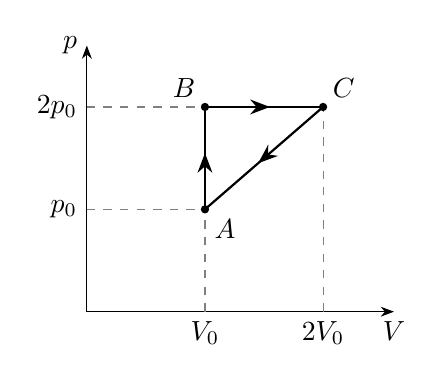
\begin{tikzpicture}[x=1.5cm,y=1.3cm]
    \draw[-{Stealth}] (0,0) -- (2.6,0) node[below] {$V$};
    \draw[-{Stealth}] (0,0) -- (0,2.6) node[left] {$p$};
    \draw[dashed,gray] (1,0) node[below,black] {$V_0$} -- (1,1);
    \draw[dashed,gray] (2,0) node[below,black] {$2V_0$} -- (2,2);
    \draw[dashed,gray] (0,1) node[left,black] {$p_0$} -- (1,1);
    \draw[dashed,gray] (0,2) node[left,black] {$2p_0$} -- (1,2);
    \draw[thick,midarrow] (1,1) -- (1,2);
    \draw[thick,midarrow] (1,2) -- (2,2);
    \draw[thick,midarrow] (2,2) -- (1,1);
    \foreach \p/\n/\pos in {{(1,1)}/A/below right, {(1,2)}/B/above left,
                            {(2,2)}/C/above right}
      \fill \p circle (1.5pt) node[\pos] {$\n$};
  \end{tikzpicture}
\end{minipage}
  \begin{enumerate}
    \item Hány mól gáz végzi a körfolyamatot? Mekkora a hőmérséklet a $B$ és a $C$
      állapotban?
    \item Nevezd meg a szakaszokat! Számold ki szakaszonként a gázon végzett munkát, a
      belső energia megváltozását és a közölt hőt ($p_0V_0$ egységben és joule-ban is)!
      \emph{Tipp: a $C\to A$ szakaszon a munkát a görbe alatti területből, a hőt az
      I.~főtételből kapod.}
    \item Ellenőrizd, hogy a teljes körfolyamatra $\Delta E = 0$!
    \item Mennyi a felvett hő és a hasznos munka? A hasznos munkát két módon is határozd
      meg! Mekkora a hatásfok?
    \item Mekkora lenne a hatásfok felső korlátja a körfolyamat legmagasabb és legalacsonyabb
      hőmérséklete között? Mit jelent az összehasonlítás?
    \item A 4.~órán ugyanezen az $A$, $B$, $C$ ponton átmenő téglalap-körfolyamatot
      vizsgáltuk (a negyedik csúcs $D\,(p_0, 2V_0)$ volt), és $\eta = 2/13$ jött ki. Miért
      ugyanannyi a felvett hő a két esetben, és miért fele akkora a hatásfok?
    \item Ábrázold az $A\to B$ és a $B\to C$ szakaszt $V$--$T$ diagramon!
      \emph{(Szorgalmi: milyen alakú a $C\to A$ szakasz a $V$--$T$ diagramon?)}
    \item Milyen gép lenne a körfolyamatból, ha fordított irányban járnánk körbe? Mennyi
      munkát kellene befektetni ciklusonként?
  \end{enumerate}

\item \textbf{Jégkocka a fagyasztóban.} A fagyasztóba $0{,}5$~kg $20\,^\circ$C-os vizet
  teszünk, amelyből $0\,^\circ$C-os jég lesz. A fagyasztó belsejében $-18\,^\circ$C van, a
  hátoldalán lévő hőleadó rács $40\,^\circ$C-os, a konyha $20\,^\circ$C-os. A fagyasztó
  hűtési tényezője $\varepsilon = Q_\text{fel}/W = 3$.
  \begin{enumerate}
    \item Mennyi hőt kell elvonni a víztől?
    \item Vázold a víz hőmérséklet--idő grafikonját egyenletes hőelvonás mellett! Melyik
      szakasz a hosszabb, és nagyjából hányszor? Mi történik a belső energiával a
      vízszintes szakaszon?
    \item Mennyi elektromos munkát használ fel ehhez a fagyasztó, és mennyi hőt ad le a
      konyhának?
    \item Ellenőrizd, hogy a $3$-as hűtési tényező nem sérti-e a II.~főtételt!
    \item A kompresszorban a hűtőközeget gyorsan összenyomják, közben felmelegszik. Milyen
      folyamattal modellezhetjük ezt? Add meg $Q$, $W$, $\Delta E$ és $\Delta T$ előjelét!
    \item Hűl vagy melegszik egy zárt konyha, ha nyitva hagyjuk a hűtőszekrény ajtaját?
      Indokold energiamérleggel!
    \item Valaki azt javasolja: a hátoldalon leadott hővel hajtsunk egy hőerőgépet, amely a
      konyha levegőjébe adja le a hulladékhőt, és a kompresszort működteti. Így a fagyasztó
      ,,ingyen'' működne. Mutasd meg számolással, hogy ez nem lehetséges! Milyen perpetuum
      mobile lenne ez, és melyik főtételt sértené?
  \end{enumerate}
\end{enumerate}

\end{document}
